\documentclass[conference]{IEEEtran}
\IEEEoverridecommandlockouts

% 1. Ρυθμίσεις Γλωσσών (XeLaTeX/LuaLaTeX)
\usepackage[greek,english]{babel}
\usepackage{fontspec}

% 2. Επιλογή Γραμματοσειράς - GFS Artemisia (Η καλύτερη για ελληνική διπλωματική)
\babelfont{rm}{GFS Artemisia}
\babelfont[greek]{rm}{GFS Artemisia}
% The preceding line is only needed to identify funding in the first footnote. If that is unneeded, please comment it out.
\usepackage{cite}
\usepackage{amsmath,amssymb,amsfonts}
\usepackage{graphicx}
\usepackage{textcomp}
\usepackage{xcolor}
\def\BibTeX{{\rm B\kern-.05em{\sc i\kern-.025em b}\kern-.08em
    T\kern-.1667em\lower.7ex\hbox{E}\kern-.125emX}}
\begin{document}

\title{Προκαταρκτική Διερεύνηση και Εκτίμηση Ταλαντωτικών Ιδιομορφών στο Σύστημα Δύο Περιοχών (Kundur) μέσω Ανάλυσης Ringdown και της Μεθόδου Matrix Pencil}

\author{
    \IEEEauthorblockN{Γεωργανάκης Νικόλαος}
    \IEEEauthorblockA{\textit{Τμήμα Ηλεκτρολόγων Μηχανικών και Μηχανικών Υπολογιστών} \\
    \textit{Αριστοτέλειο Πανεπιστήμιο Θεσσαλονίκης }\\
    Θεσσαλονίκη, Ελλάδα}
    \and
    \IEEEauthorblockN{Επίβλεψη:}
    \IEEEauthorblockA{\textit{Θεόφιλος Παπαδόπουλος, Αν. Καθηγητής} \\
    \textit{Αχιλλέας Σφέτκος, Υποψήφιος Διδάκτορας}}
}
\maketitle

\begin{abstract}
Η παρούσα εργασία εξετάζει την εκτίμηση των ηλεκτρομηχανικών ταλαντώσεων στο σύστημα δύο περιοχών του Kundur , χρησιμοποιώντας την μέθοδο ταυτοποίησης Matrix Pencil (MP). Μέσω δυναμικών προσομοιώσεων ringdown στο περιβάλλον PowerFactory , αναλύεται ένα ευρύ σύνολο σημάτων ($V$, $I$, $P$, $Q$) από όλες τις γεννήτριες του συστήματος. Η μελέτη επικεντρώνεται στην εξαγωγή και τον χαρακτηρισμό των κυρίαρχων διασυνδετικών (inter-area) και τοπικών (intra-area) ιδιομορφών. Τα αποτελέσματα αναδεικνύουν την υψηλή πιστότητα της μεθόδου στην ανακατασκευή των αποκρίσεων, με τους δείκτες $R^2$ και RMSE να επιβεβαιώνουν την ακρίβεια της ταυτοποίησης. Η ανάλυση των ταυτοποιημένων ιδιοτιμών στο μιγαδικό επίπεδο πιστοποιεί την δυναμική ευστάθεια του συστήματος , αναδεικνύοντας παράλληλα την επίδραση της παραμετροποίησης του αλγορίθμου στην ποιότητα της εκτίμησης.
\end{abstract}

\begin{IEEEkeywords}
Matrix Pencil Method, Kundur Two-Area System, Modal Analysis, Ringdown Response, Power System Identification
\end{IEEEkeywords}

\section{Εισαγωγή}
Στην συγκεκριμένη αναφορά αναλύονται τα αποτελέσματα της ταυτοποίησης συστήματος μέσω της μεθόδου Matrix Pencil (MP) που εφαρμόστηκε στις αποκρίσεις ringdown που προέκυψαν από τη δυναμική προσομοίωση του συστήματος Kundur Two-Area. Η μελέτη επικεντρώνεται στην ανάλυση των σημάτων τάσης ($V$), ρεύματος ($I$), ενεργού ($P$) και άεργου ($Q$) ισχύος των γεννητριών $G_1$-$G_4$, με σκοπό την εκτίμηση των κυρίαρχων ταλαντωτικών ιδιομορφών (inter-area και intra-area modes) του συστήματος.


\section{Διαδικασία Παραγωγής Δεδομένων}
\subsection{Δυναμική Προσομοίωση στο PowerFactory}

Το πρώτο βήμα υλοποίησης περιελάμβανε την εισαγωγή του Kundur Two-Area System (πρότυπο μοντέλο για τη μελέτη ηλεκτρομηχανικών ταλαντώσεων) στο περιβάλλον του PowerFactory. Για τη δημιουργία των απαραίτητων χρονοσειρών, εκτελέστηκε δυναμική προσομοίωση στο πεδίο του χρόνου (RMS Simulation). Αρχικά, υπολογίστηκαν οι αρχικές συνθήκες του συστήματος (Initial Conditions) για την επίλυση της ροής φορτίου και την εξασφάλιση της μόνιμης κατάστασης λειτουργίας.

Ως συμβάν διαταραχής (event) για τη διέγερση των ηλεκτρομηχανικών ταλαντώσεων, ορίστηκε η αποσύνδεση (outage) μίας εκ των κρίσιμων γραμμών μεταφοράς που συνδέουν τις δύο περιοχές (tie-lines) τη χρονική στιγμή $t = 0$ s. Η γραμμή παρέμεινε εκτός λειτουργίας για ένα χρονικό διάστημα $1$ s, μετά το οποίο πραγματοποιήθηκε η αυτόματη επανασύνδεση της ($t = 1$ s). Η συνολική διάρκεια της προσομοίωσης ορίστηκε στα $50$ s με χρονικό βήμα ολοκλήρωσης (step size) $0.01$ s, επιτρέποντας την πλήρη καταγραφή της απόκρισης ελεύθερης ταλάντωσης (ringdown) καθώς το σύστημα τείνει προς ένα νέο σημείο ισορροπίας. Για την παρακολούθηση του φαινομένου, εξήχθησαν σε μορφή αρχείων CSV οι μεταβλητές τάσης ($V$), ρεύματος ($I$), ενεργού ($P$) και άεργου ($Q$) ισχύος για καθεμία από τις τέσσερις γεννήτριες του συστήματος ($G_1$-$G_4$).

\subsection{Προεπεξεργασία Σημάτων (Signal Pre-processing)}
Πριν την εφαρμογή του αλγορίθμου Matrix Pencil, τα πρωτογενή δεδομένα του PowerFactory υποβλήθηκαν σε απαραίτητη ψηφιακή επεξεργασία (μέσω της γλώσσας Python), προκειμένου να εξασφαλιστεί η αξιοπιστία της ταυτοποίησης. Τα στάδια της προεπεξεργασίας περιελάμβαναν:

\begin{enumerate}
    \item \textbf{Αποκοπή Χρονοσειρών:} Διατηρήθηκαν τα δεδομένα για $t > 1.2$ s, αφήνοντας ένα περιθώριο ασφαλείας $0.2$ s μετά την επανασύνδεση της γραμμής. Αυτό απομονώνει την καθαρή ringdown απόκριση από τα μεταβατικά φαινόμενα των διακοπτών.
    \item \textbf{Αφαίρεση Μόνιμης Συνιστώσας (Detrending):} Αφαιρέθηκε η DC συνιστώσα (offset), μετατοπίζοντας την ταλάντωση γύρω από το μηδέν.
    \item \textbf{Φιλτράρισμα (Filtering):} Εφαρμόστηκε βαθυπερατό φίλτρο (Low-Pass) με συχνότητα αποκοπής $f_{c} = 10$ Hz για την απομάκρυνση υψίσυχνου θορύβου.
\end{enumerate}
\section{Μαθηματική Ανακατασκευή Σημάτων}

\subsection{Εφαρμογή της Μεθόδου Matrix Pencil (MP)}
Η διαδικασία της ταυτοποίησης βασίστηκε στην ανάλυση των προεπεξεργασμένων σημάτων $V$, $I$, $P$ και $Q$ μέσω του αλγορίθμου Matrix Pencil. Σύμφωνα με τις απαιτήσεις της διερεύνησης, η μέθοδος εφαρμόστηκε με δύο διαφορετικές προσεγγίσεις για τον καθορισμό της τάξης του συστήματος ($n$):

\begin{enumerate}
    \item \textbf{Καθορισμένη Τάξη:} Χρησιμοποιήθηκαν σταθερές τιμές τάξης $n \in \{2, 4, 6\}$, ώστε να αξιολογηθεί η ικανότητα της μεθόδου να περιγράψει το σύστημα με περιορισμένο αριθμό πόλων.
    \item \textbf{Αυτόματος Καθορισμός Τάξης:} Εφαρμόστηκε η τεχνική της αποκοπής των ιδιοτιμών με παραμέτρους ανοχής $\tau \in \{1, 0.1, 0.01\}$, επιτρέποντας στον αλγόριθμο να επιλέξει αυτόματα τον αριθμό των κυρίαρχων ιδιομορφών ανάλογα με το ενεργειακό περιεχόμενο του σήματος.
\end{enumerate}

\subsection{Μαθηματική Ανακατασκευή και Πιστότητα}
Για κάθε σενάριο ταυτοποίησης εξήχθησαν οι παράμετροι των ιδιομορφών: το πλάτος ($A_{i}$), ο ρυθμός απόσβεσης ($\sigma_{i}$), η συχνότητα ($f_{i}$ σε Hz) και η φάση ($\varphi_{i}$). Η μαθηματική ανακατασκευή του σήματος $\hat{y}(t)$ πραγματοποιήθηκε μέσω της σχέσης:

\begin{equation}
\hat{y}(t)=\sum_{i=1}^{n}A_{i}e^{\sigma_{i}t}\cos(2\pi f_{i}t+\varphi_{i})
\label{eq:reconstruction}
\end{equation}

Η πιστότητα της ανακατασκευής αξιολογήθηκε μέσω του συντελεστή προσδιορισμού $R^{2}$ και του μέσου τετραγωνικού σφάλματος RMSE. Η διαδικασία αυτή εξασφαλίζει ότι οι ταυτοποιημένες ιδιομορφές αντιπροσωπεύουν με ακρίβεια τη φυσική απόκριση του συστήματος Kundur και δεν αποτελούν μαθηματικά σφάλματα της προσέγγισης.



\section{Αποτελέσματα και Γραφικές Παραστάσεις}
\subsection{Απεικόνιση Παραμέτρων Ιδιομορφών (Real Part vs Frequency)}
Ως αποτέλεσμα της εφαρμογής του αλγορίθμου Matrix Pencil, ελήφθησαν τα διαγράμματα της παρούσας παραγράφου, στα οποία παρουσιάζεται η κατανομή των ιδιομορφών στο μιγαδικό επίπεδο για τα μετρούμενα μεγέθη των γεννητριών του συστήματος. Συγκεκριμένα, στον οριζόντιο άξονα παρουσιάζεται ο ρυθμός απόσβεσης ($\sigma$), ο οποίος αποτελεί το πραγματικό μέρος των ιδιοτιμών, ενώ στον κατακόρυφο άξονα η συχνότητα ταλάντωσης ($f$) σε Hz.

\begin{figure}[htbp]
    \centering
    
\includegraphics[width=0.8\linewidth]{./plots/modal_maps/g1_2x2_grid.png} 
    \caption{Κατανομή ιδιοτιμών (Real Part vs Frequency) για τη γεννήτρια $G_1$.}
    \label{fig:poles_distribution_g1}
\end{figure}

\begin{figure}[htbp]
    \centering
    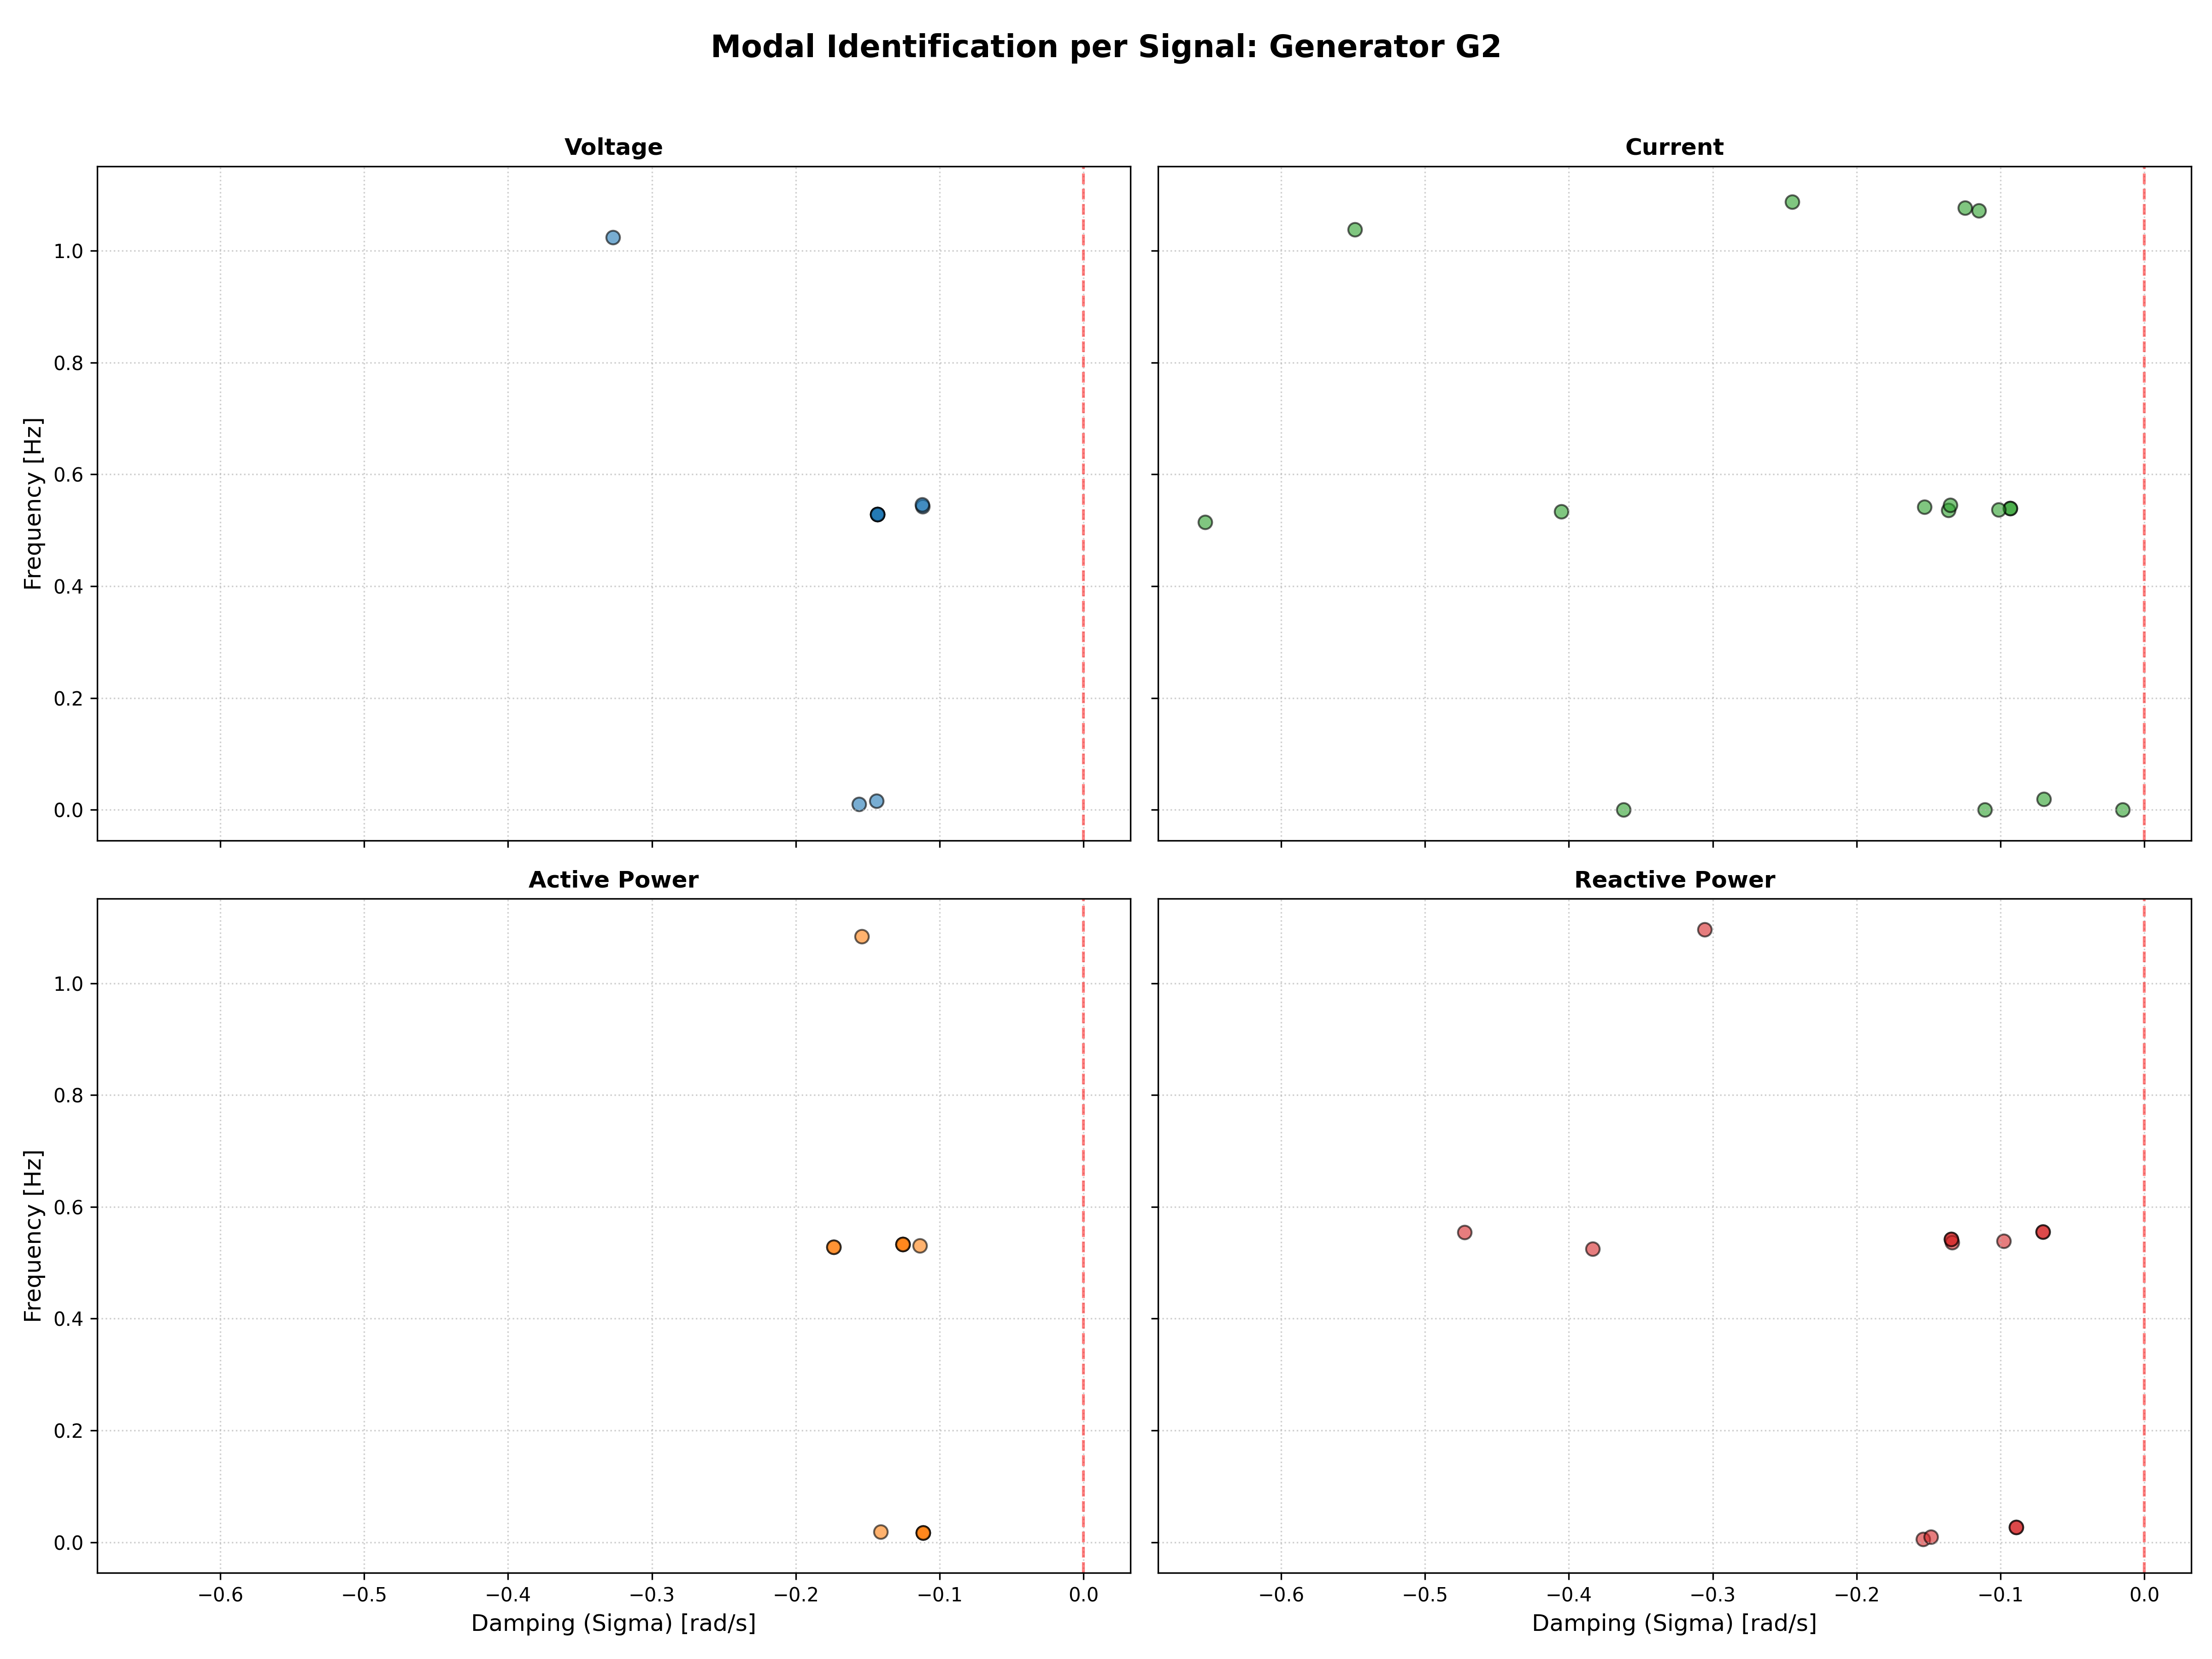
\includegraphics[width=0.8\linewidth]{./plots/modal_maps/g2_2x2_grid.png} 
    \caption{Κατανομή ιδιοτιμών (Real Part vs Frequency) για τη γεννήτρια $G_2$.}
    \label{fig:poles_distribution_g2}
\end{figure}

\begin{figure}[htbp]
    \centering
    
\includegraphics[width=0.8\linewidth]{./plots/modal_maps/g3_2x2_grid.png} 
    \caption{Κατανομή ιδιοτιμών (Real Part vs Frequency) για τη γεννήτρια $G_3$.}
    \label{fig:poles_distribution_g3}
\end{figure}

\begin{figure}[htbp]
    \centering
    
\includegraphics[width=0.8\linewidth]{./plots/modal_maps/g4_2x2_grid.png} 
    \caption{Κατανομή ιδιοτιμών (Real Part vs Frequency) για τη γεννήτρια $G_4$.}
    \label{fig:poles_distribution_g4}
\end{figure}

\begin{figure}[htbp]
    \centering
    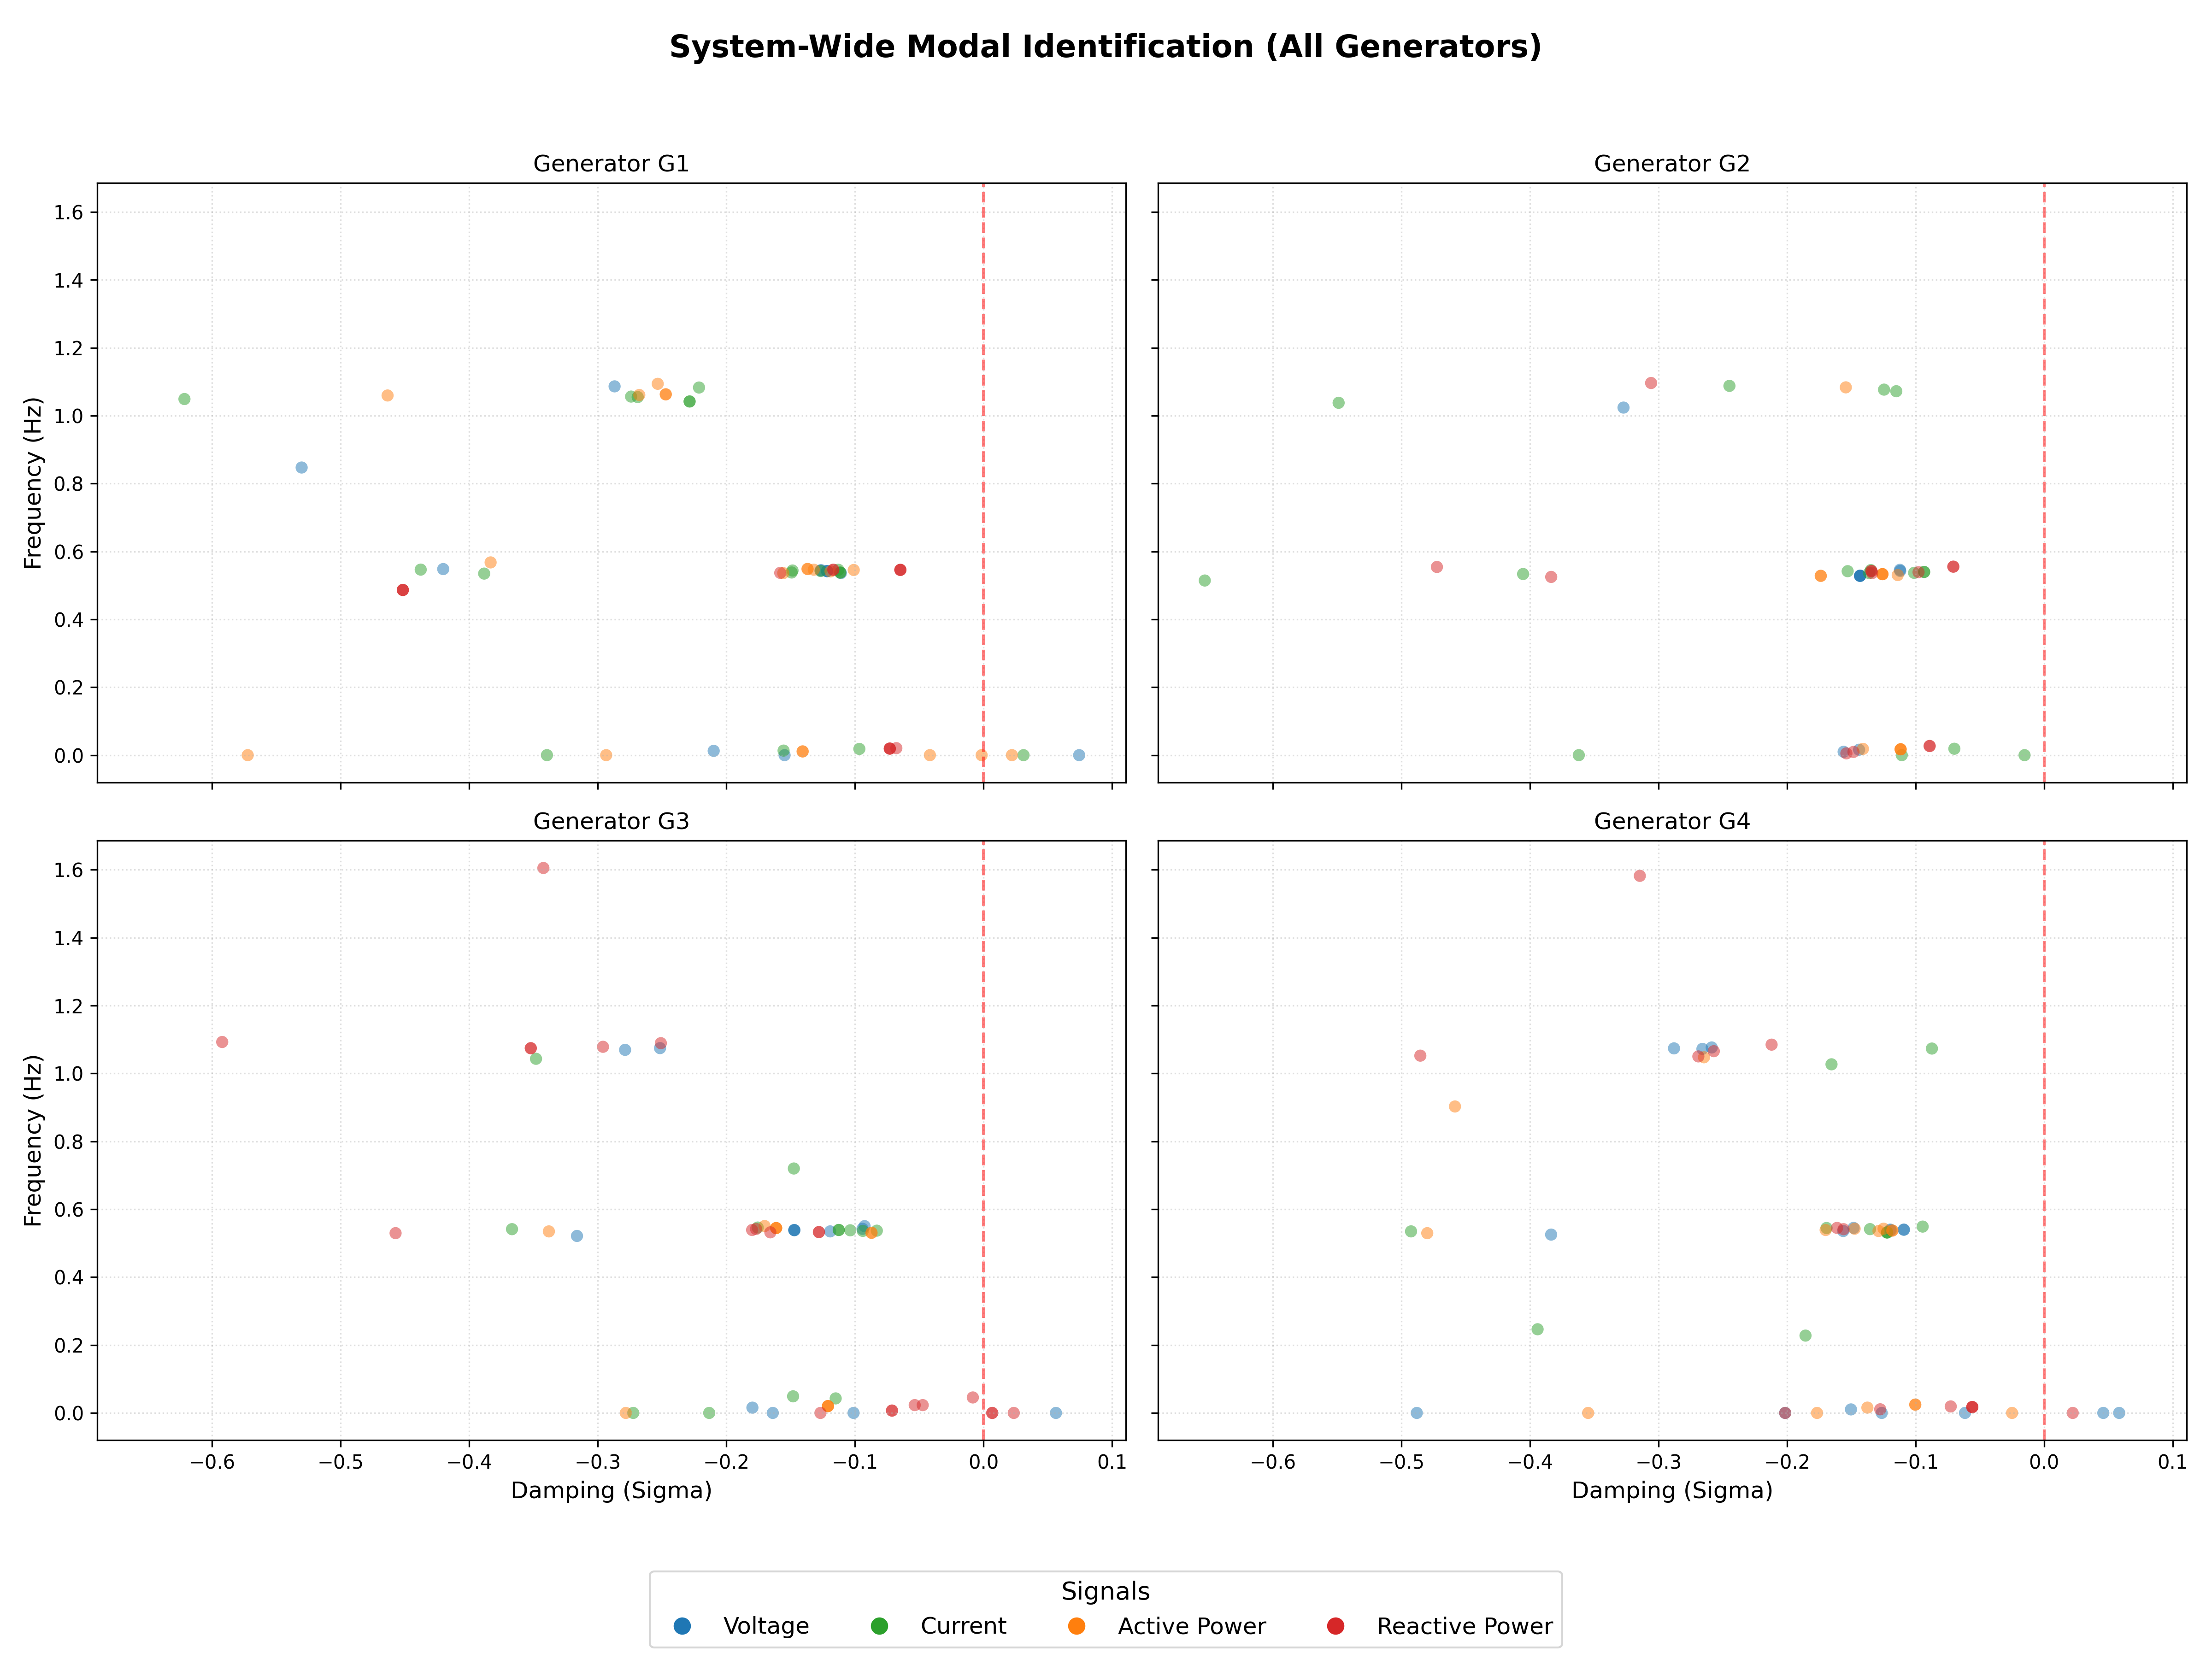
\includegraphics[width=0.8\linewidth]{./plots/modal_maps/All_Generators_Grid.png} 
    \caption{Κατανομή ιδιοτιμών (Real Part vs Frequency) για τις γεννήτριες $G_1$-$G_4$.}
    \label{fig:poles_distribution_all}
\end{figure}

Στα γραφήματα αποτυπώνεται η κατανομή των ταυτοποιημένων ιδιοτιμών για τις τέσσερις γεννήτριες του συστήματος ($G_1$-$G_4$), συσχετίζοντας τη συχνότητα ταλάντωσης (Hz) με τον ρυθμό απόσβεσης ($\sigma$). Η ανάλυση επιβεβαιώνει την ευστάθεια του συστήματος, καθώς το σύνολο σχεδόν των σημείων εντοπίζεται στο αριστερό ημιεπίπεδο (αρνητικό $\sigma$), υποδεικνύοντας τη θετική απόσβεση των ταλαντώσεων. Ιδιαίτερα σημαντική είναι η έντονη ομαδοποίηση σημείων στην περιοχή των $0.5$-$0.6$ Hz, η οποία εμφανίζεται ομοιόμορφα σε όλες τις γεννήτριες και σε όλα τα καταγεγραμμένα σήματα ($V$, $I$, $P$, $Q$), αποτελώντας ένδειξη του κύριου τρόπου ταλάντωσης (inter-area) του συστήματος Kundur. Επιπρόσθετα, διακρίνονται διακριτές συστάδες στην περιοχή του $1.0$ έως $1.2$ Hz, οι οποίες αντιστοιχούν στις τοπικές ταλαντώσεις (intra-area) των μηχανών εντός της εκάστοτε περιοχής. Πέρα αυτών, καταγράφονται στον οριζόντιο άξονα και ιδιοτιμές με μηδενική συχνότητα. Αυτές αντιστοιχούν σε μη ταλαντωτικά φαινόμενα ή προκύπτουν ως διορθωτικοί πόλοι του αλγορίθμου για την αντιστάθμιση υπολειπόμενων μόνιμων συνιστωσών (DC offsets) στα σήματα.

\subsection{Αξιολόγηση Πιστότητας Ανακατασκευής (Signal Reconstruction)}
Για την επαλήθευση της εγκυρότητας των ιδιομορφών που εξήχθησαν στην προηγούμενη ενότητα, πραγματοποιήθηκε μαθηματική ανακατασκευή των σημάτων στο πεδίο του χρόνου. Αρχικά, εξετάστηκε η συμπεριφορά των επιμέρους προσεγγίσεων (σταθερής τάξης $n$ και ανοχής $\tau$) προκειμένου να αξιολογηθεί η επίδραση τους στην ακρίβεια της προσαρμογής.

\begin{figure}[htbp]
    \centering
    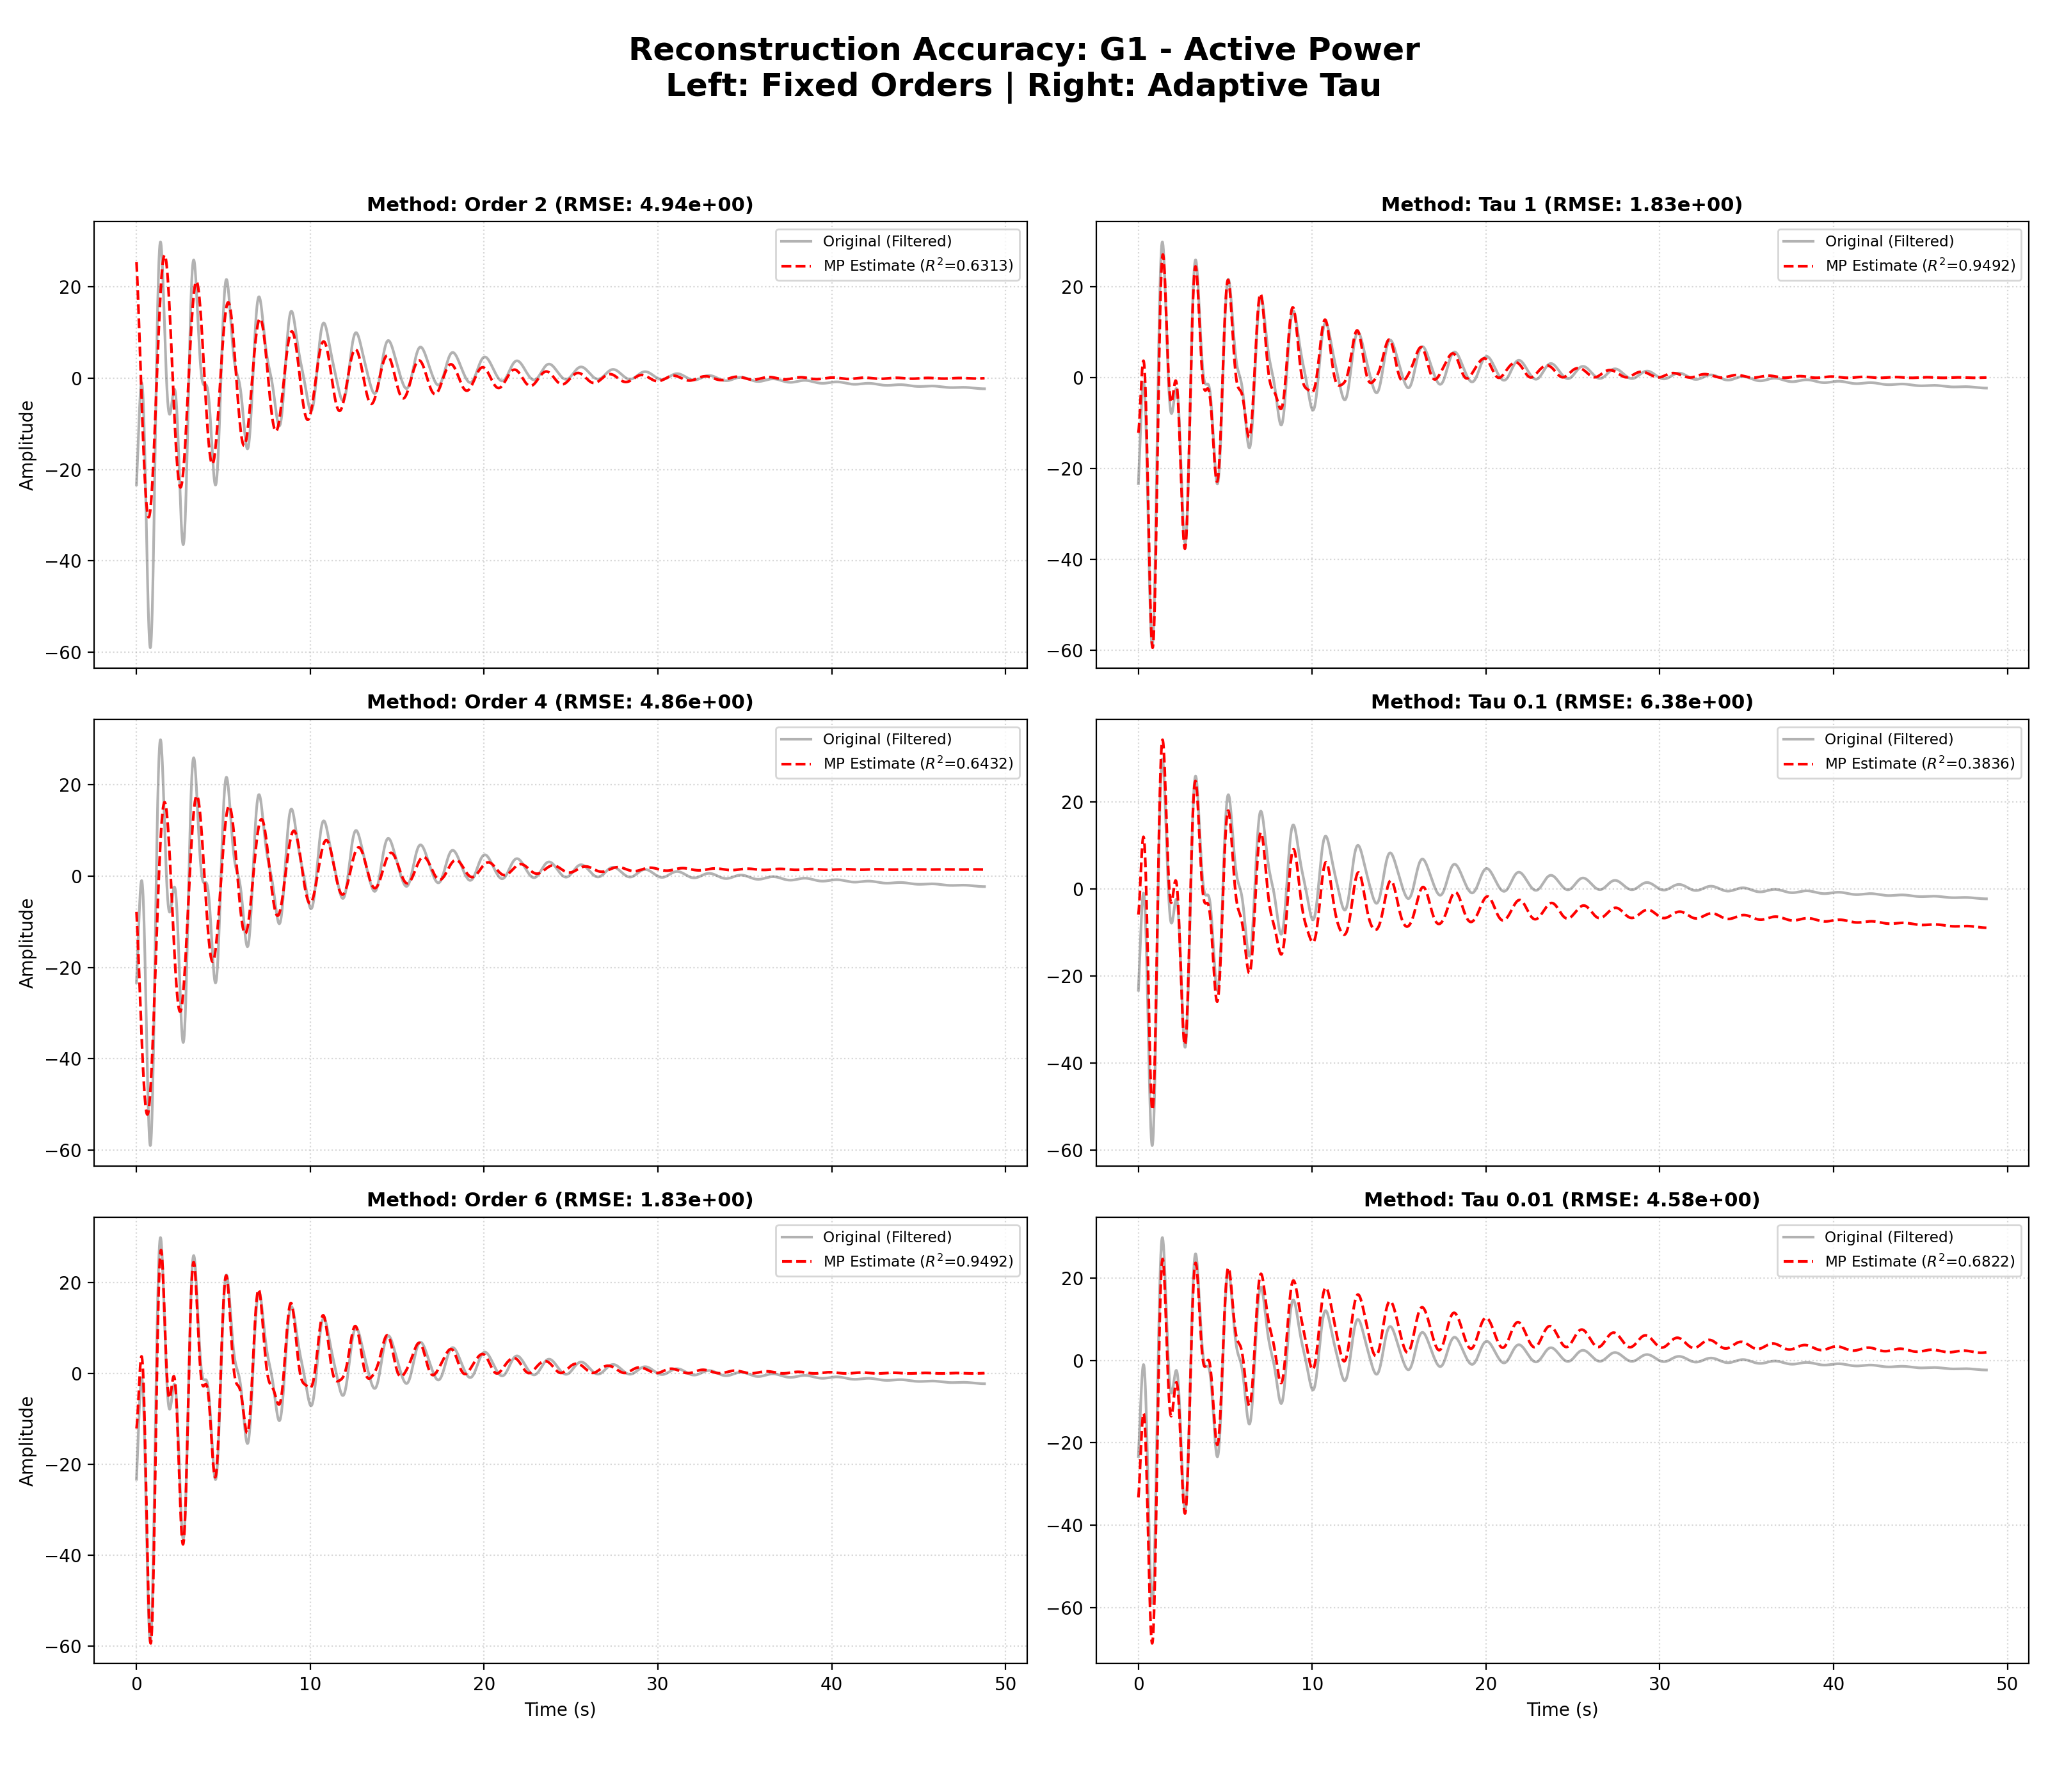
\includegraphics[width=0.8\linewidth]{./plots/reconstruction_grids/g1_Active_Power_Reconstruction.png} 
    \caption{Ανακατασκευή σήματος ενεργής ισχύος ($P$) για τη γεννήτρια $G_1$.}
    \label{fig:g1_active_power_reconstruction}
\end{figure}

Στη συνέχεια δημιουργήθηκε ένα συγκεντρωτικό γράφημα το οποίο αποτυπώνει την άμεση σύγκριση μεταξύ των αρχικών σημάτων (Original Filtered) και των αντίστοιχων εκτιμώμενων (MP estimate) επιλέγοντας αυστηρά την παραμετροποίηση που απέδωσε την υψηλότερη ακρίβεια (Max $R^2$) για το εκάστοτε σήμα.

\begin{figure}[htbp]
    \centering
    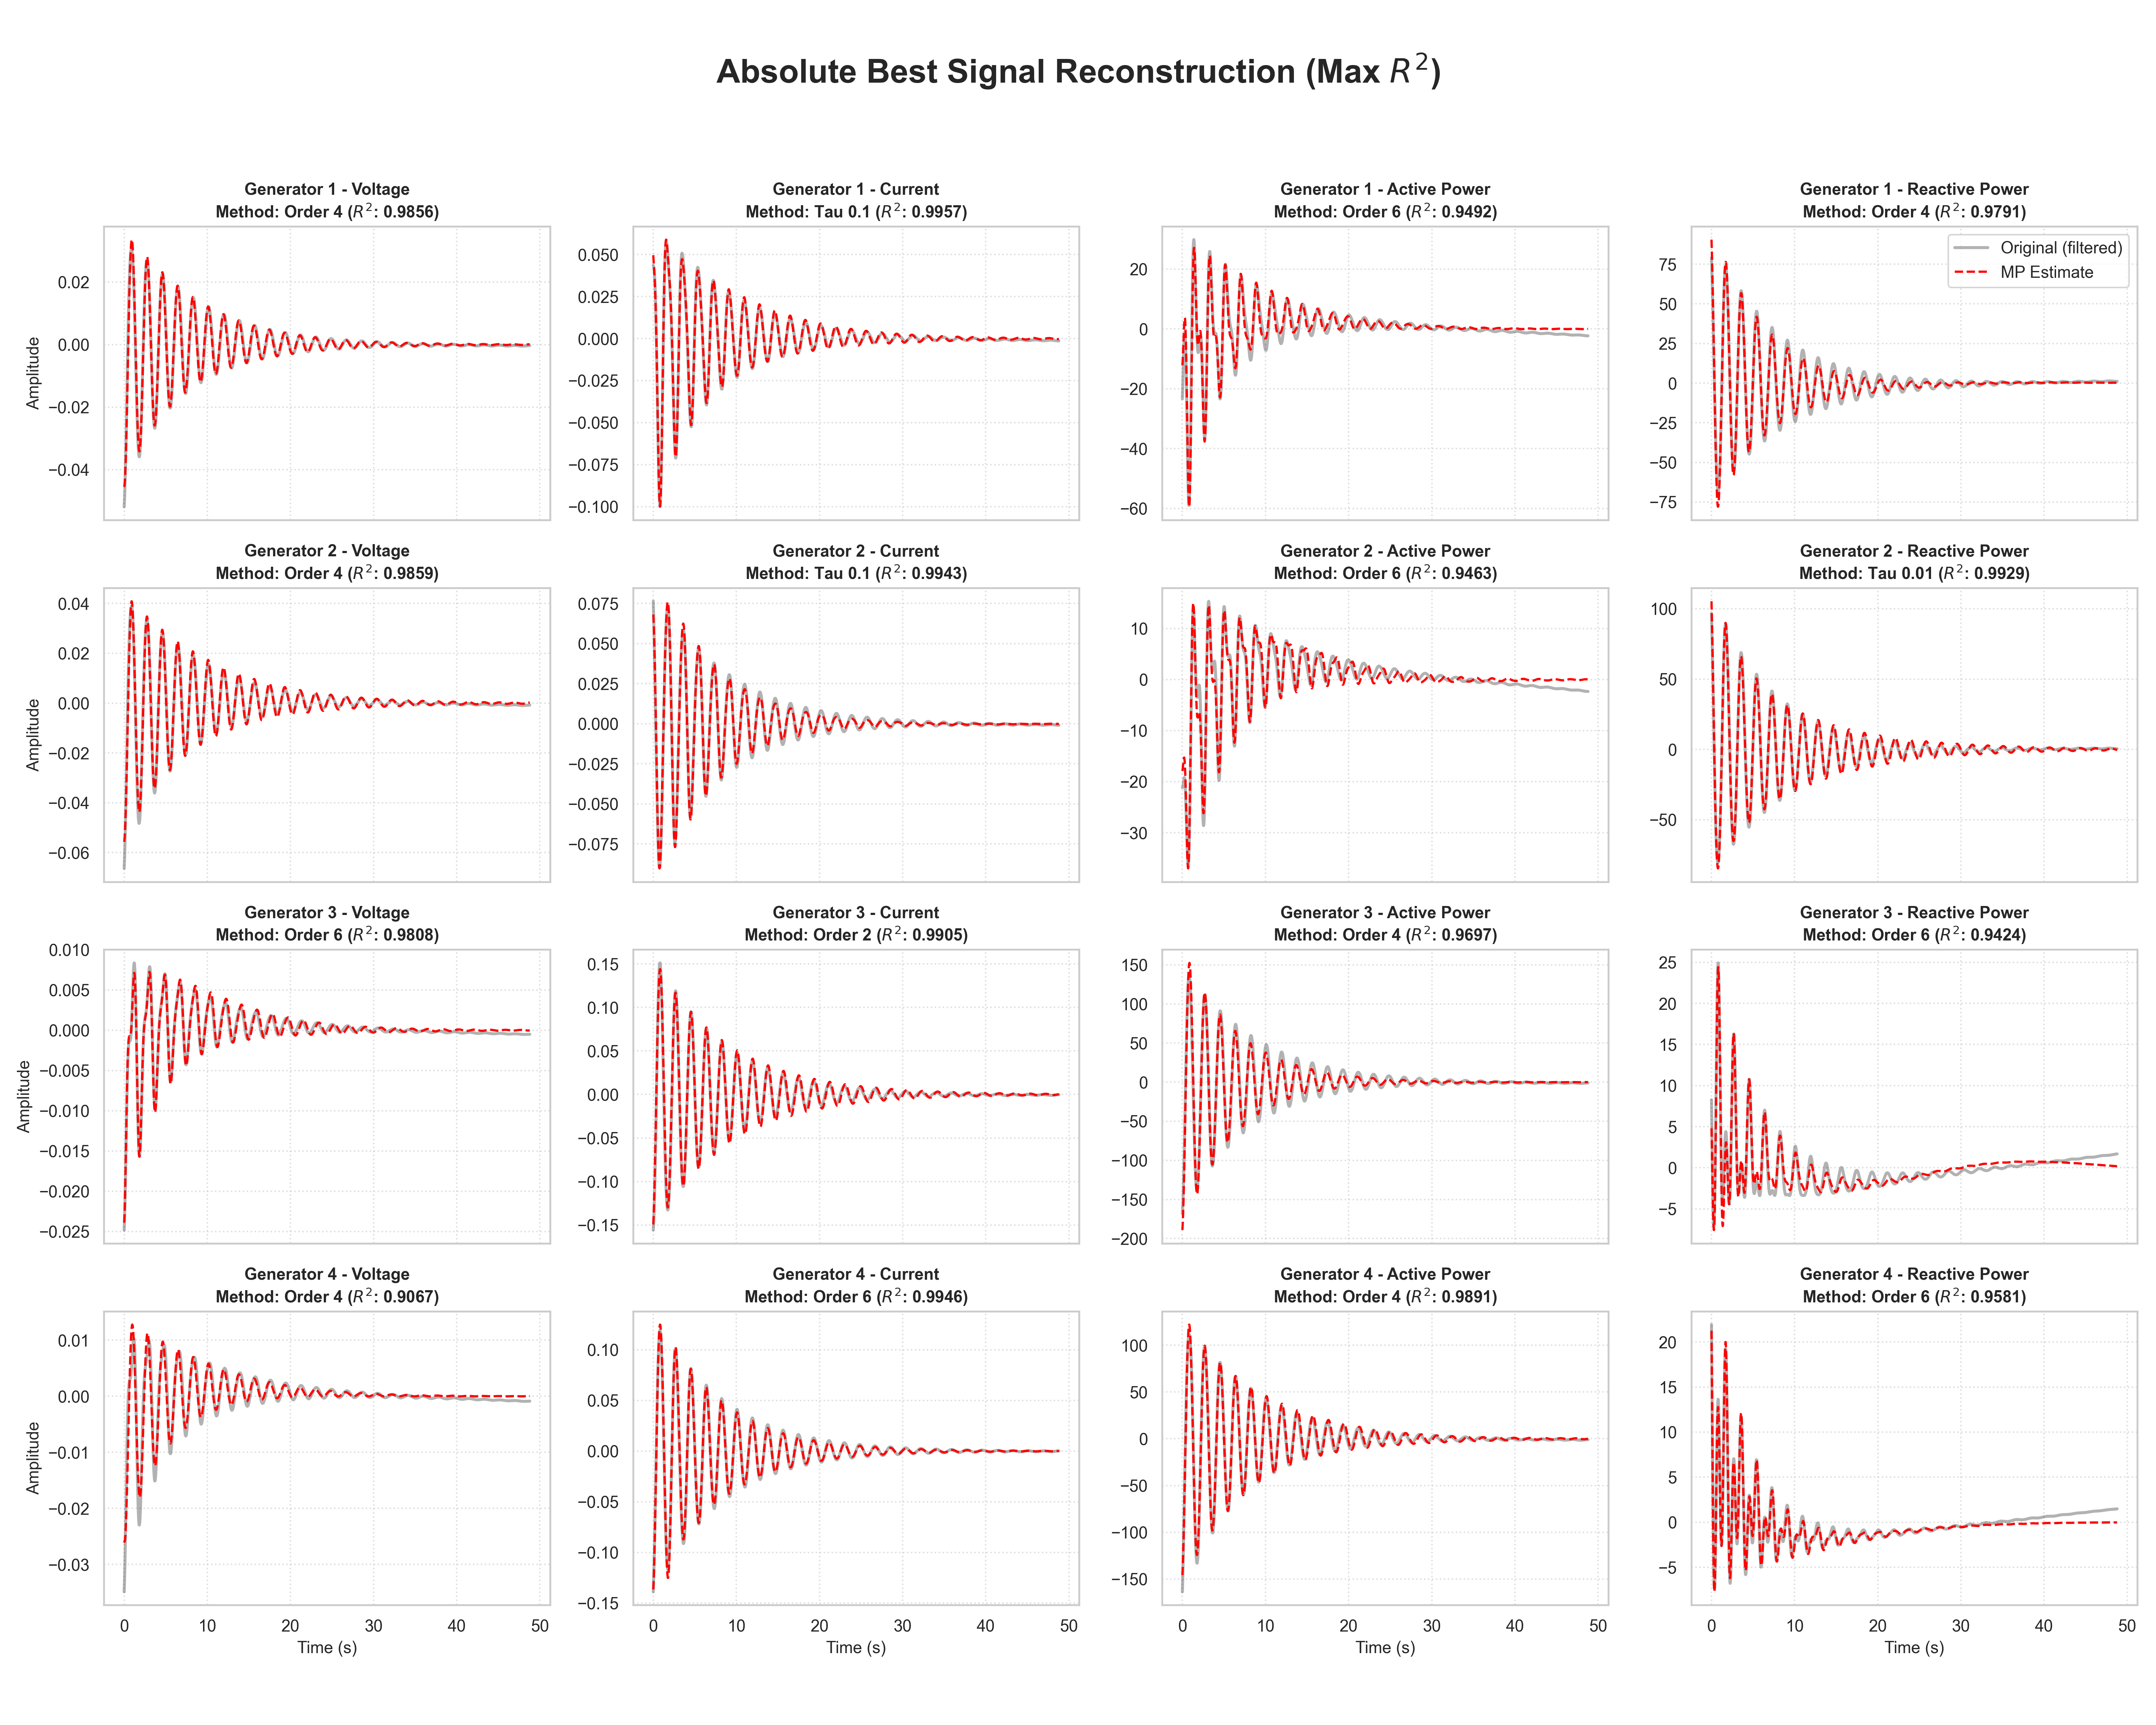
\includegraphics[width=0.8\linewidth]{./stats/9_best_reconstruction_grid.png} 
    \caption{Βέλτιστη μαθηματική ανακατασκευή των σημάτων ($V, I, P, Q$) για τις γεννήτριες $G_1$-$G_4$ με βάση το μέγιστο συντελεστή προσδιορισμού $R^2$.}
    \label{fig:best_reconstrution}
\end{figure}

Όπως παρατηρείται, επιτυγχάνεται εξαιρετική σύμπτωση των δύο κυματομορφών σε όλες τις εξεταζόμενες γεννήτριες, ωστόσο αξίζει να σημειωθεί ότι η βέλτιστη ανακατασκευή δεν προκύπτει από μία καθολική μέθοδο γεγονός που επιβεβαιώνει την αναγκαιότητα εξέτασης πολλαπλών προσεγγίσεων.

Τέλος, η ταύτιση των κυματομορφών αναλύεται στο χρονικό παράθυρο της ελεύθερης ταλάντωσης (ringdown), το οποίο ξεκινά μετά την εκκαθάριση της διαταραχής (περίπου στα $1.2$ s). Το προαναφερθέν γεγονός επιβεβαιώνει την ορθή εφαρμογή της διαδικασίας απόρριψης των αρχικών δειγμάτων και του βαθυπερατού φίλτρου. 

\subsection{Ταυτοποίηση Κυρίαρχων Ταλαντώσεων (Συνολική Αξιολόγηση)}
Η συνολική αξιολόγηση της δυναμικής του συστήματος πραγματοποιήθηκε μέσω της συνδυαστικής μελέτης των στατιστικών κατανομών και των χαρτών ιδιομορφών.

\textbf{Ανάλυση Πυκνότητας Πόλων (Heatmap)}
Μέσω του Pole Density Heatmap, αποτυπώνεται το πλήθος των ιδιοτιμών που εντόπισε ο αλγόριθμος ανά γεννήτρια και ανά είδος σήματος. Παρατηρείται ότι η άεργος ισχύς ($Q$) της γεννήτριας $G_3$ παρουσιάζει την μέγιστη πυκνότητα ιδιοτιμών, ενώ στην γεννήτρια $G_1$ την μεγαλύτερη πυκνότητα έχουν τα σήματα ρεύματος ($I$) και ενεργού ισχύος ($P$). Η διαφοροποίηση αυτή υποδεικνύει ότι τα συγκεκριμένα σήματα λειτουργούν ως οι πλέον κατάλληλες πηγές πληροφορίας για τη συμπεριφορά του δικτύου.

\begin{figure}[htbp]
    \centering
    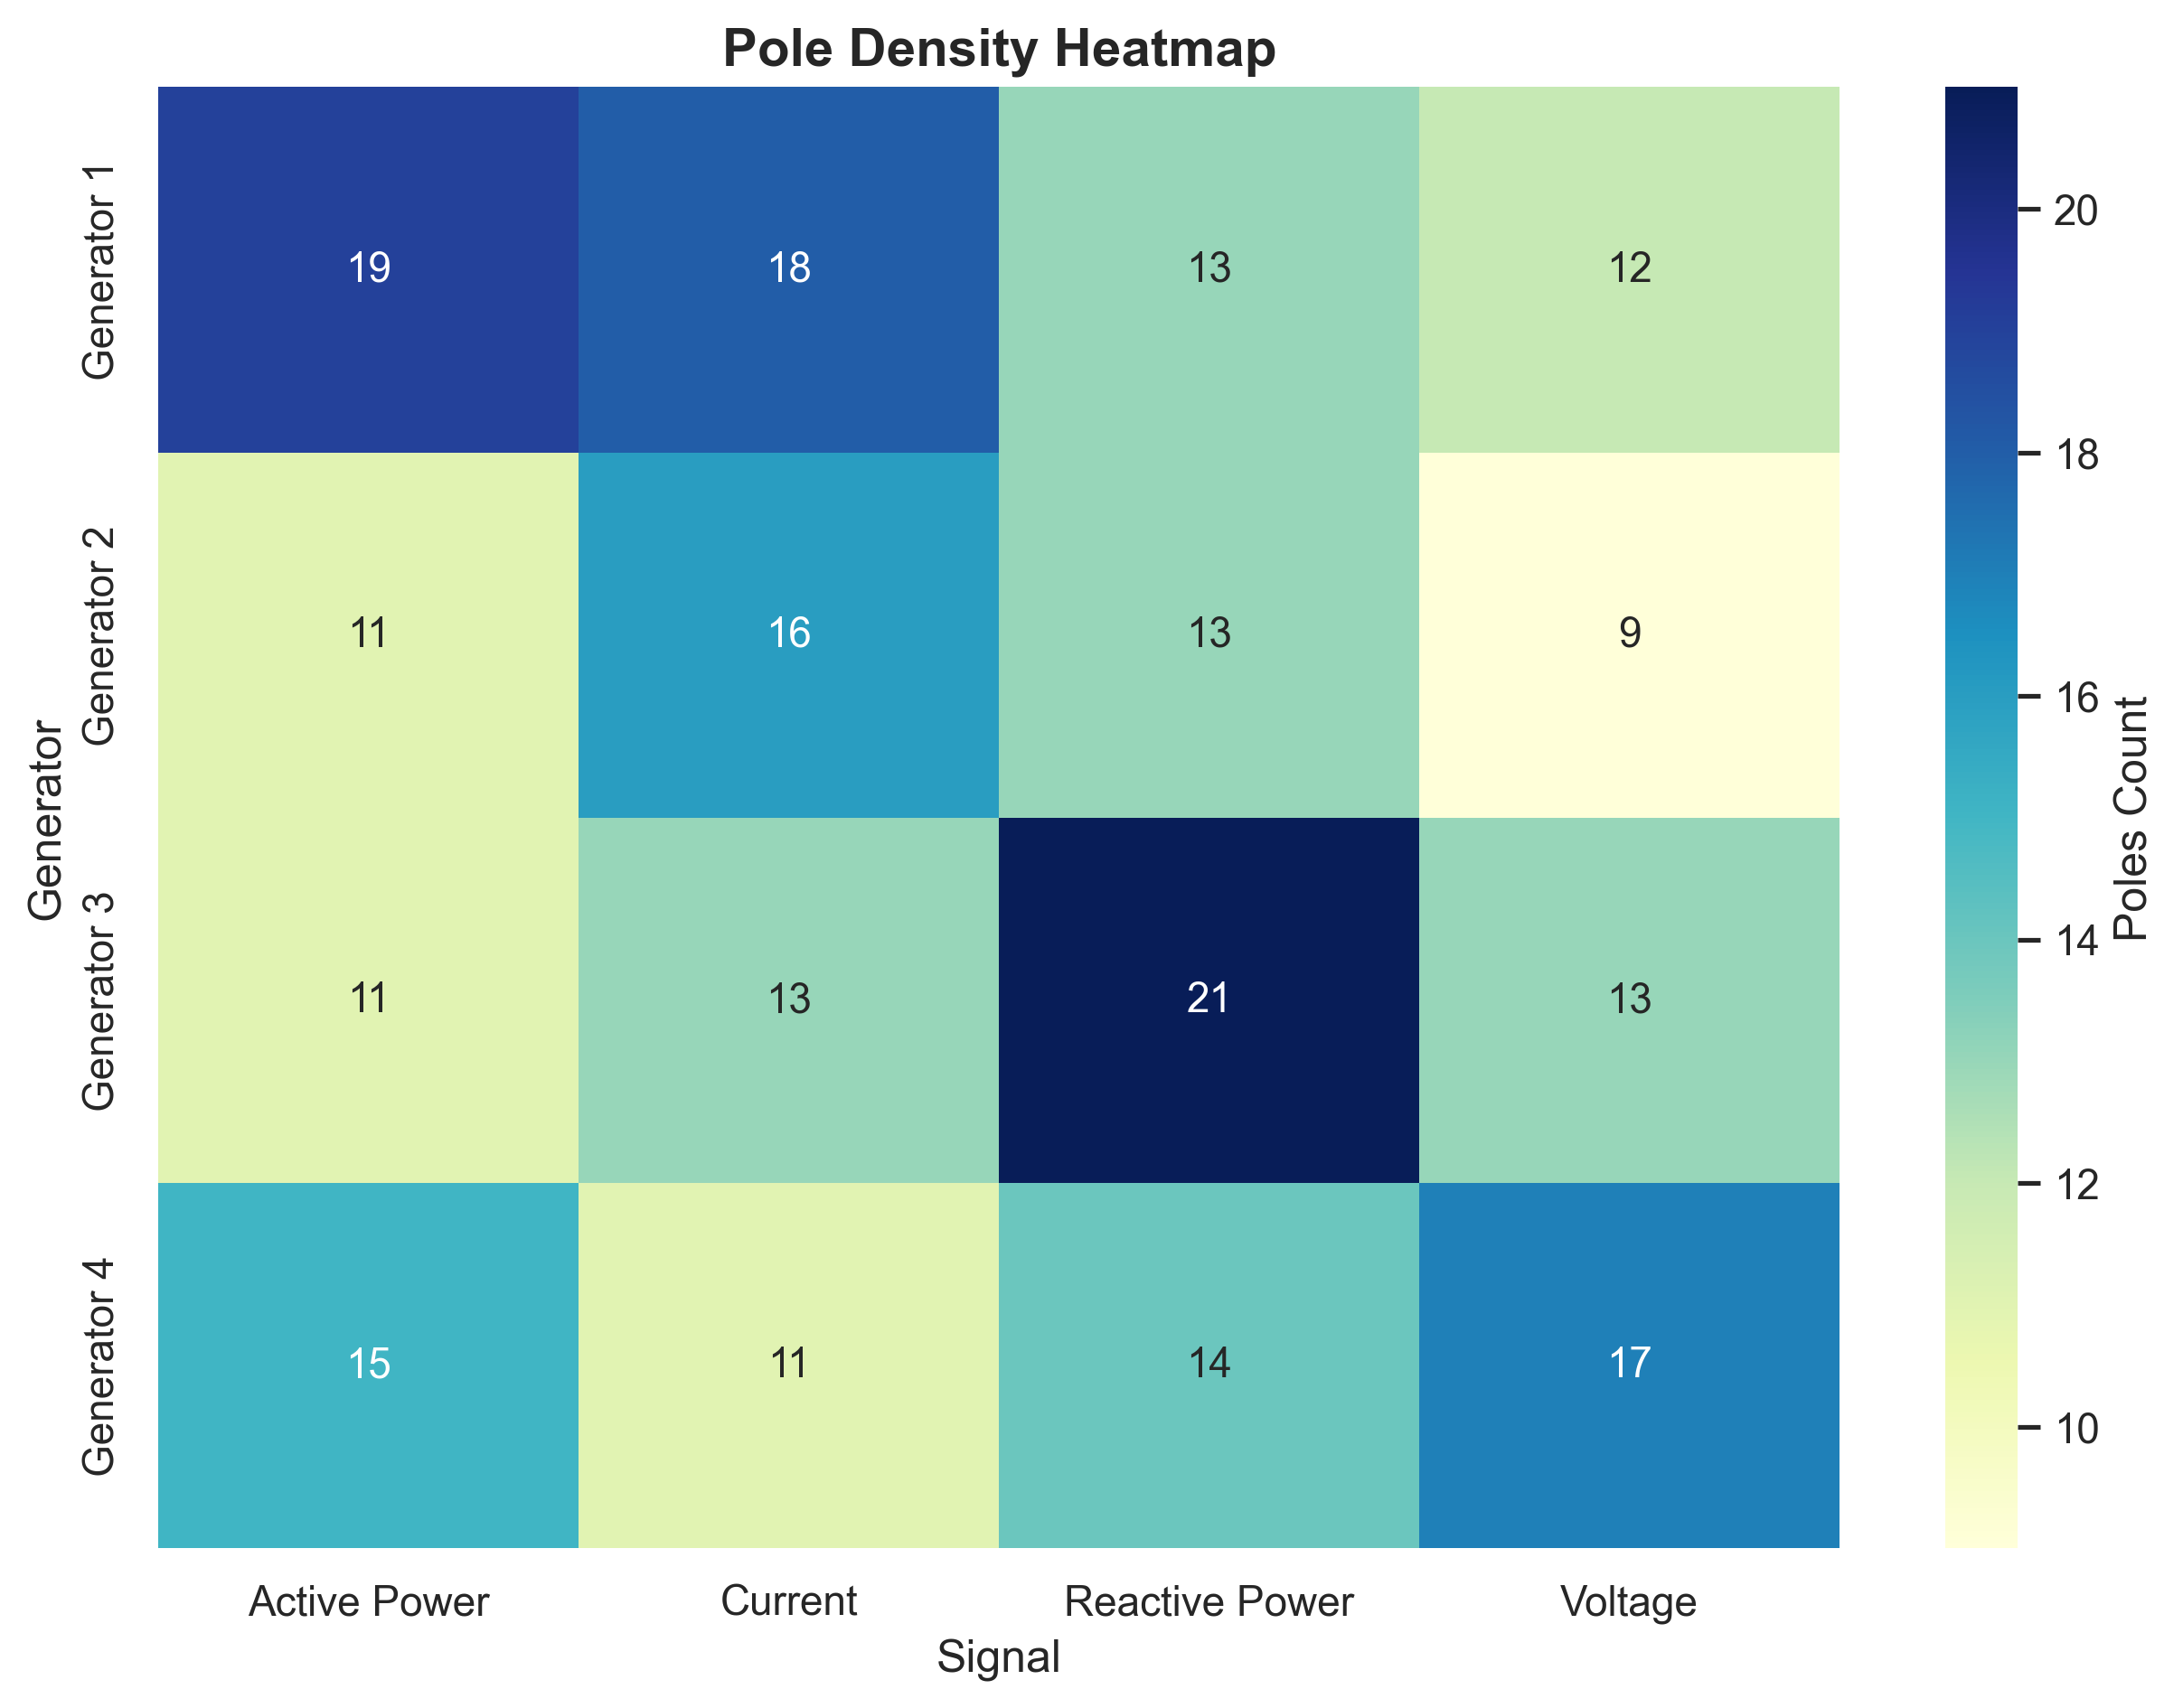
\includegraphics[width=\linewidth]{./stats/1_heatmap.png}
    \caption{Χάρτης πυκνότητας πόλων ανά γεννήτρια και μετρούμενο μέγεθος.}
    \label{fig:heatmap}
\end{figure}

\textbf{Χάρτης Ιδιομορφών (Bubble Map)}
Η ανάλυση του Model Frequency/Damping Map παρέχει τη πληρέστερη εικόνα της ταυτοποίησης και επιβεβαιώνει πλήρως τα ευρήματα που παρουσιάστηκαν στην ενότητα 4.1. Το μέγεθος κάθε “φυσαλίδας” είναι ανάλογο με την ενέργεια (πλάτος) του αντίστοιχου τρόπου ταλάντωσης. Παρατηρείται μια σαφής κατακόρυφη ευθυγράμμιση στην περιοχή ανάμεσα στα $0.5$ με $0.6$ Hz, η οποία υποδηλώνει την παρουσία μιας inter-area ταλάντωσης. Ο συγκεκριμένος τρόπος εμφανίζει ιδιαίτερα υψηλή ένταση (μεγάλο μέγεθος φυσαλίδων), κυρίως στα σήματα της ενεργού ($P$) και άεργου ($Q$) ισχύος των γεννητριών. Παράλληλα, διακρίνεται ένας δευτερεύον τρόπος ταλάντωσης στην περιοχή των $1$ Hz με $1.2$ Hz, ο οποίος αντιστοιχεί σε τοπικές (intra-area) ταλαντώσεις. Οι ιδιομορφές αυτής της περιοχής εμφανίζουν γενικά πιο αρνητικές τιμές του ρυθμού απόσβεσης $\sigma$, γεγονός που υποδηλώνει ταχύτερη απόσβεση. Τέλος, παρατηρούνται και ιδιοτιμές κοντά στα $0$ Hz, οι οποίες αντιστοιχούν σε μη ταλαντωτικά φαινόμενα ή σε διορθωτικούς πόλους της μεθόδου για την προσαρμογή των υπολειπόμενων μόνιμων συνιστωσών των σημάτων.
\begin{figure}[htbp] % Χρήση figure* για δίστηλη απεικόνιση
    \centering
    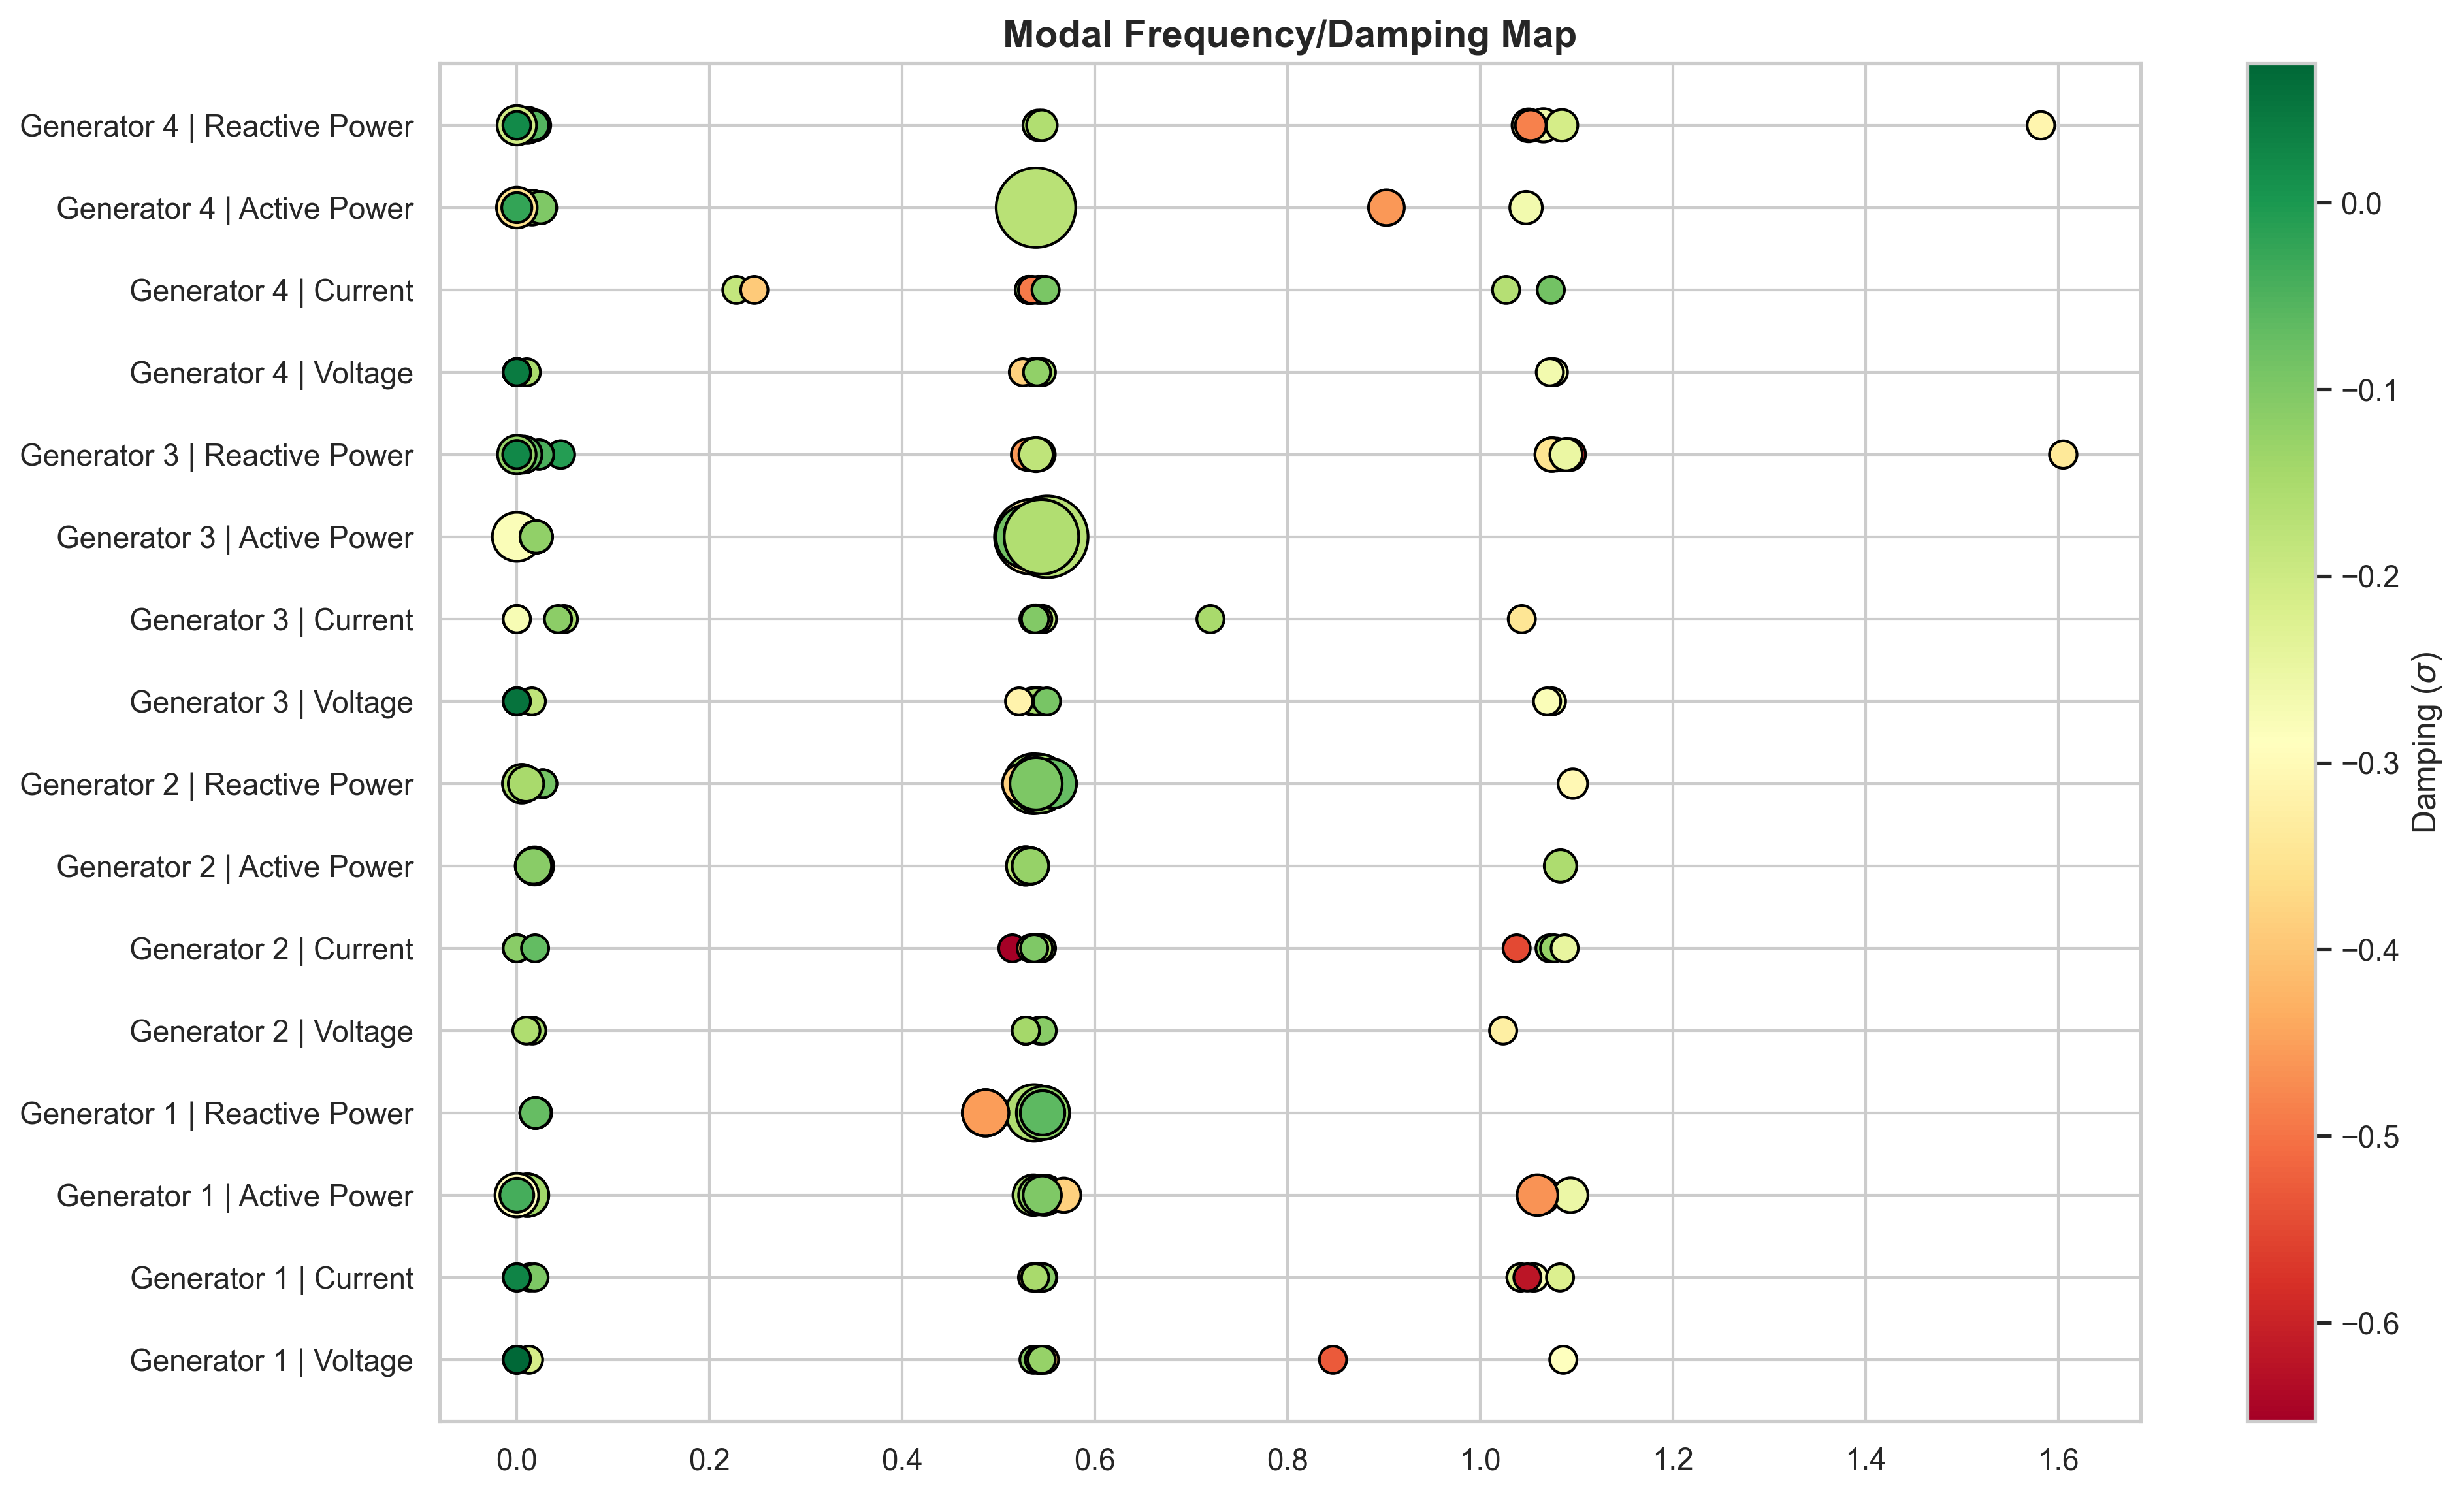
\includegraphics[width=0.9\linewidth]{./stats/5_bubble_map.png}
    \caption{Χάρτης Ιδιομορφών (Bubble Map): Συγκεντρωτική απεικόνιση συχνότητας, απόσβεσης και ενέργειας των ταυτοποιημένων modes.}
    \label{fig:bubble_map}
\end{figure}

\section{Συμπεράσματα}
Η ολοκλήρωση της προκαταρκτικής διερεύνησης επιβεβαιώνει την αξιοπιστία της μεθόδου ταυτοποίησης, με την εξαιρετική ακρίβεια στην ανακατασκευή των σημάτων να αποδεικνύει την ικανότητα του αλγορίθμου Matrix Pencil να εξάγει επιτυχώς τις ιδιοτιμές από τις ringdown αποκρίσεις. Aπό την ανάλυση προκύπτει ότι το σύστημα Kundur παραμένει ευσταθές, καθώς σχεδόν όλες οι ιδιοτιμές διαθέτουν αρνητικό πραγματικό μέρος ($\sigma < 0$). Καθοριστικό ρόλο στην ορθή έκβαση των αποτελεσμάτων είχε η χρήση βαθυπερατού φίλτρου και η επιλογή του κατάλληλου χρονικού παραθύρου μετά τη διαταραχή, εξασφαλίζοντας την μελέτη στο καθαρό σήμα. Παρά την ακρίβεια των εκτιμήσεων ανά γεννήτρια, η παρατηρούμενη μικρή διασπορά των τιμών καθιστά αναγκαία τη χρήση αλγορίθμων συσταδοποίησης (όπως ο DBSCAN) για την απομόνωση των Inter-area modes. Συνολικά, η ροή εργασίας από το PowerFactory στην Python λειτούργησε υποδειγματικά, θέτοντας τις βάσεις για την αυτοματοποιημένη παρακολούθηση της δυναμικής ευστάθειας του συστήματος σε πραγματικό χρόνο.

% \begin{thebibliography}{00}
% % Μπορείς να προσθέσεις εδώ τις δικές σου βιβλιογραφικές αναφορές (π.χ. τα,, κλπ.)
% \end{thebibliography}

\end{document}